\chapter{Summit Gear Portal}
\label{ch:portal}

The Summit Gear Portal is a comprehensive Next.js web application backed by Supabase. It serves as the central online platform for mountaineers to purchase equipment, register devices, and manage their expedition gear.

\section{Getting Started}

\subsection{Creating an Account}
To access the full features of the portal, including device registration and firmware downloads, you must create a user account.

\begin{enumerate}
    \item Navigate to \url{https://portal.summitgear.com} in your web browser.
    \item Click on the \textbf{Sign Up} button in the top right corner.
    \item Provide your name, a valid email address, and a secure password.
    \item Check your email for a verification link and click it to activate your account.
\end{enumerate}

\begin{infobox}
The portal utilizes Supabase authentication. Your data is protected by strict Row-Level Security (RLS) policies in the PostgreSQL database.
\end{infobox}

\begin{figure}[H]
    \centering
    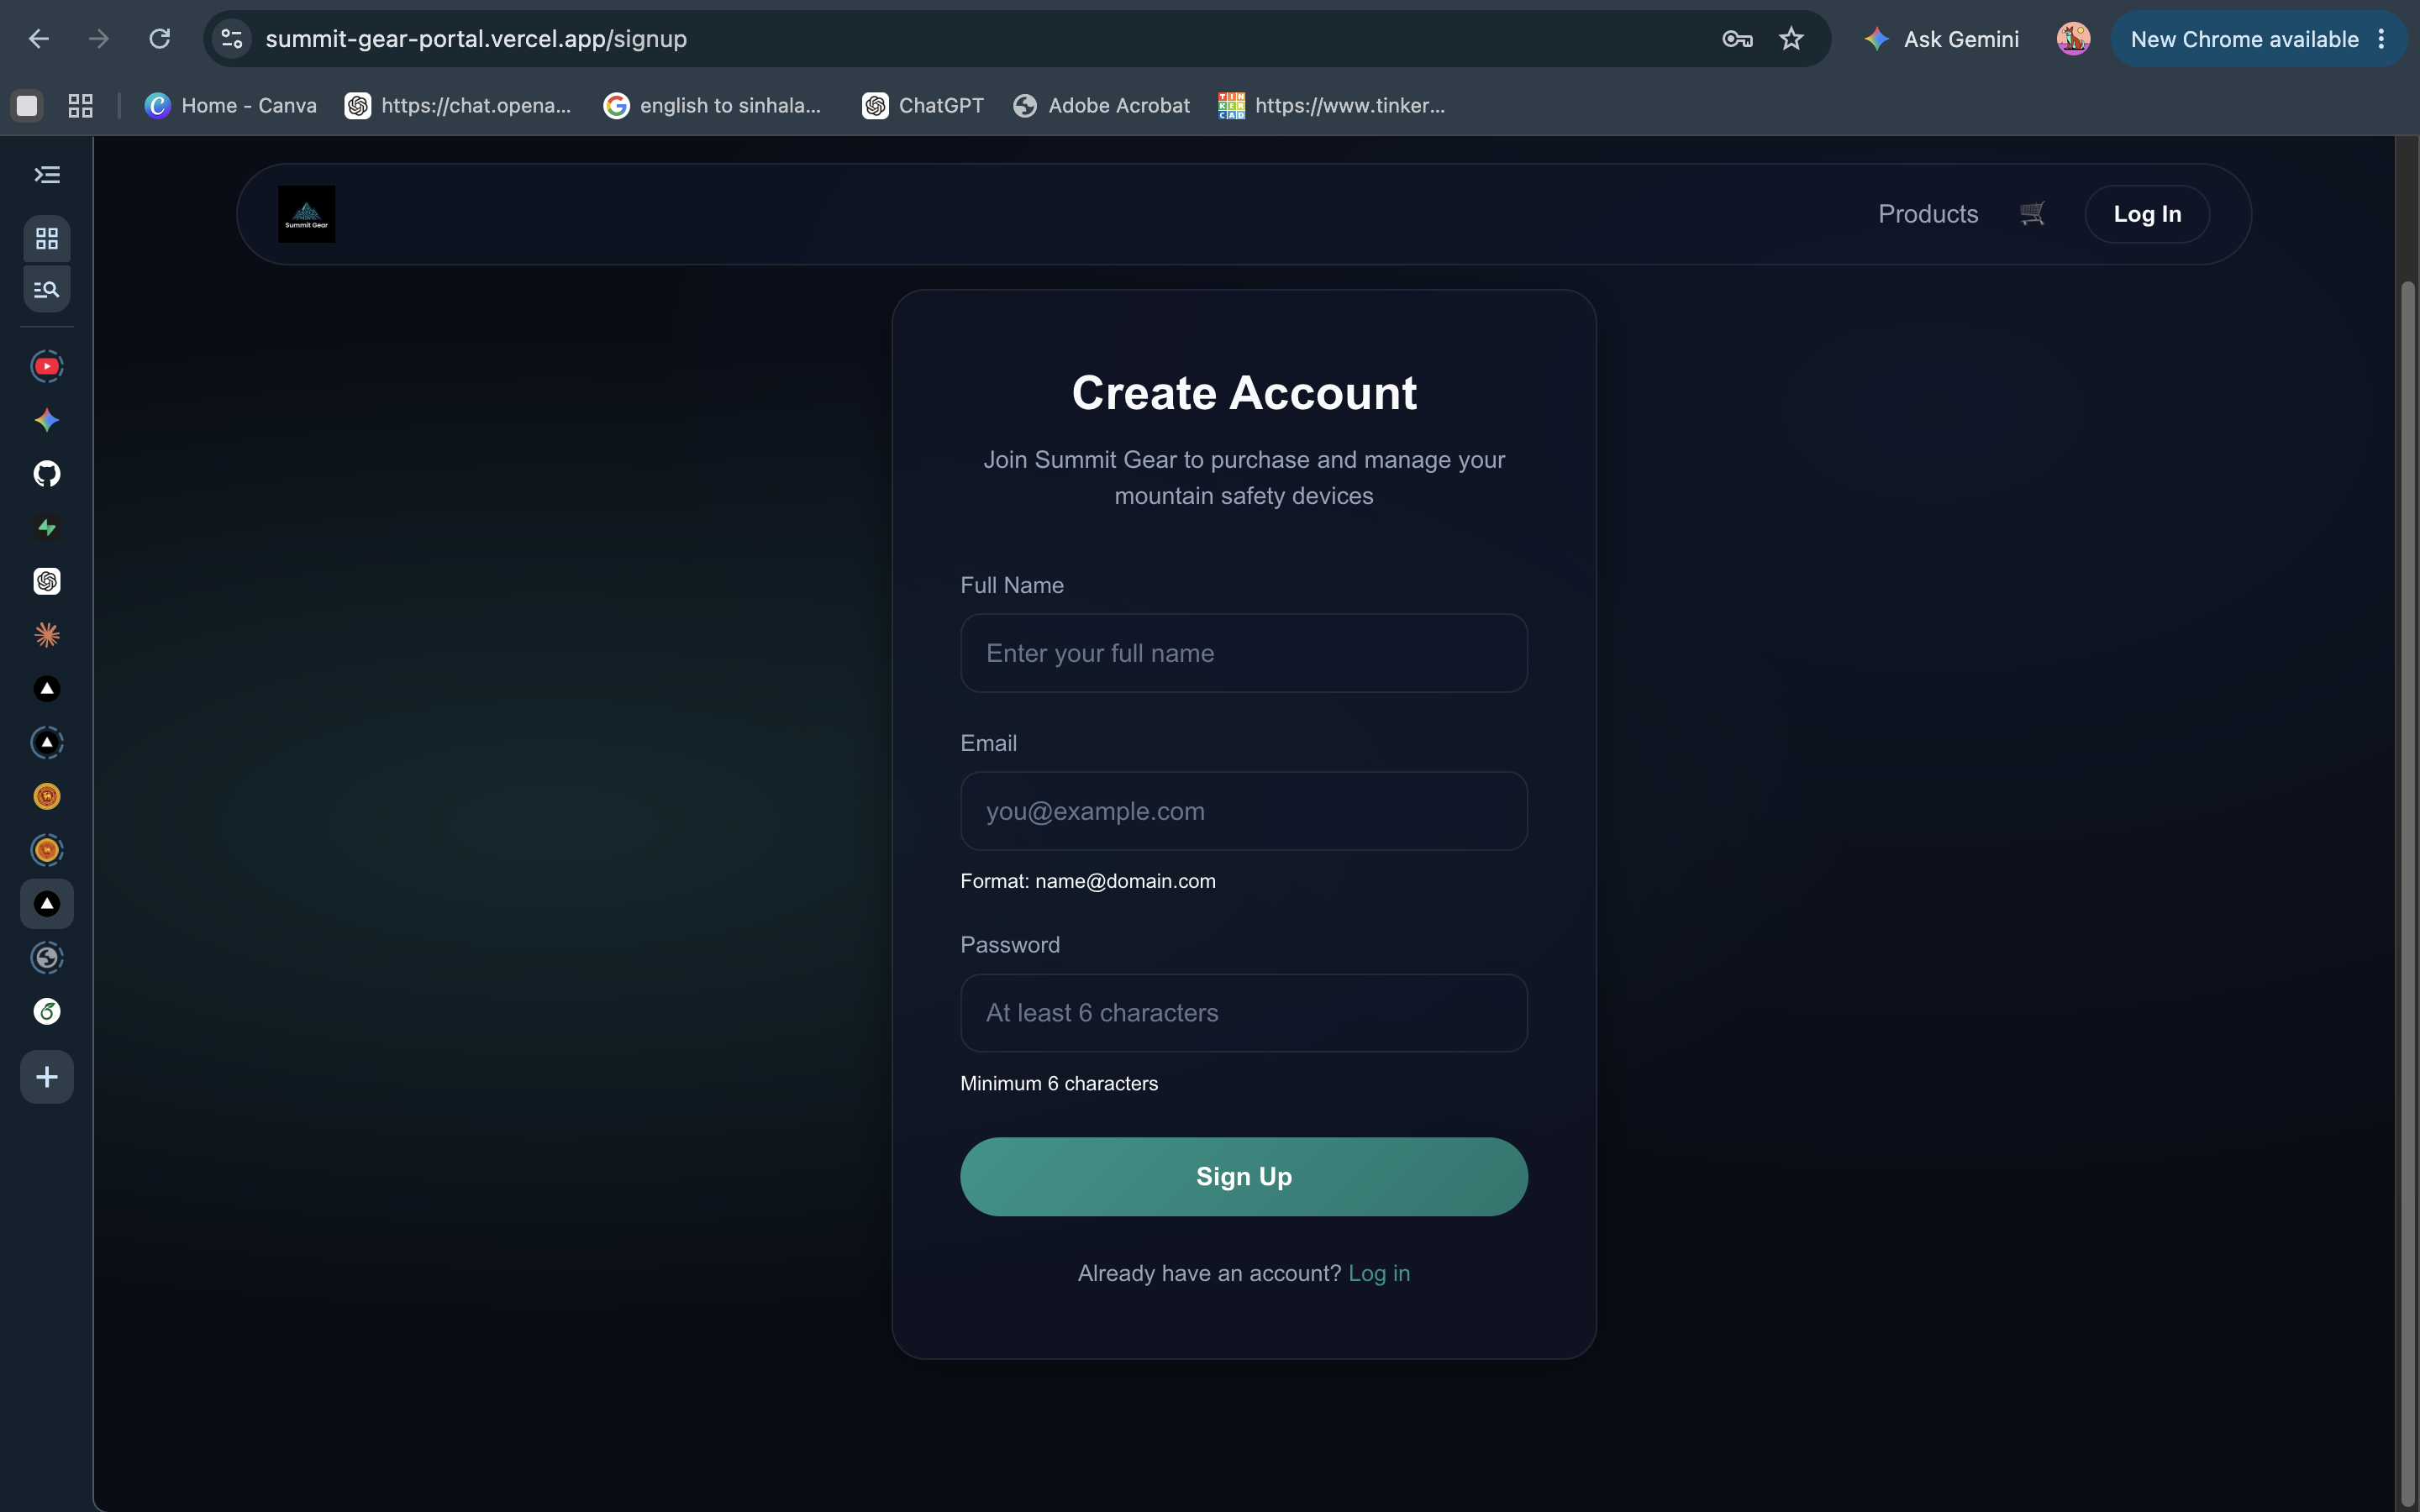
\includegraphics[width=0.8\textwidth]{figures/portal-signup.png}
    \caption{Summit Gear Portal Account Creation Page}
    \label{fig:portal-signup}
\end{figure}

\section{E-commerce Operations}

\subsection{Browsing the Product Catalog}
The portal features a full e-commerce storefront for summiting equipment.

\begin{itemize}
    \item Navigate to the \textbf{Shop} tab from the main menu.
    \item Use the category filters on the left side to narrow down products (e.g., Tracker Devices, Accessories, Apparel).
    \item Click on any product to view detailed specifications, compatibility information, and pricing.
\end{itemize}

\subsection{Adding to Cart and Checkout}
\begin{enumerate}
    \item On a product page, select your desired quantity and click \textbf{Add to Cart}.
    \item Once ready, click the Cart icon in the header to review your items.
    \item Proceed to checkout, where you will enter your shipping information and payment details.
    \item Upon successful payment, you will receive an order confirmation email containing your invoice and tracking details.
\end{enumerate}

\section{Device Management}

\subsection{Registering a Purchased Device}
To enable firmware updates and warranty support, you must register your Climber Main Device to your account.

\begin{enumerate}
    \item Log in to your account and navigate to the \textbf{My Devices} dashboard.
    \item Click \textbf{Register New Device}.
    \item Enter the unique Serial Number found on the sticker underneath the device's battery compartment.
    \item Enter the purchase date and click \textbf{Submit}.
\end{enumerate}

\begin{tipbox}
Registering your device automatically adds you to the mailing list for critical safety updates and new firmware release notifications.
\end{tipbox}

\begin{figure}[H]
    \centering
    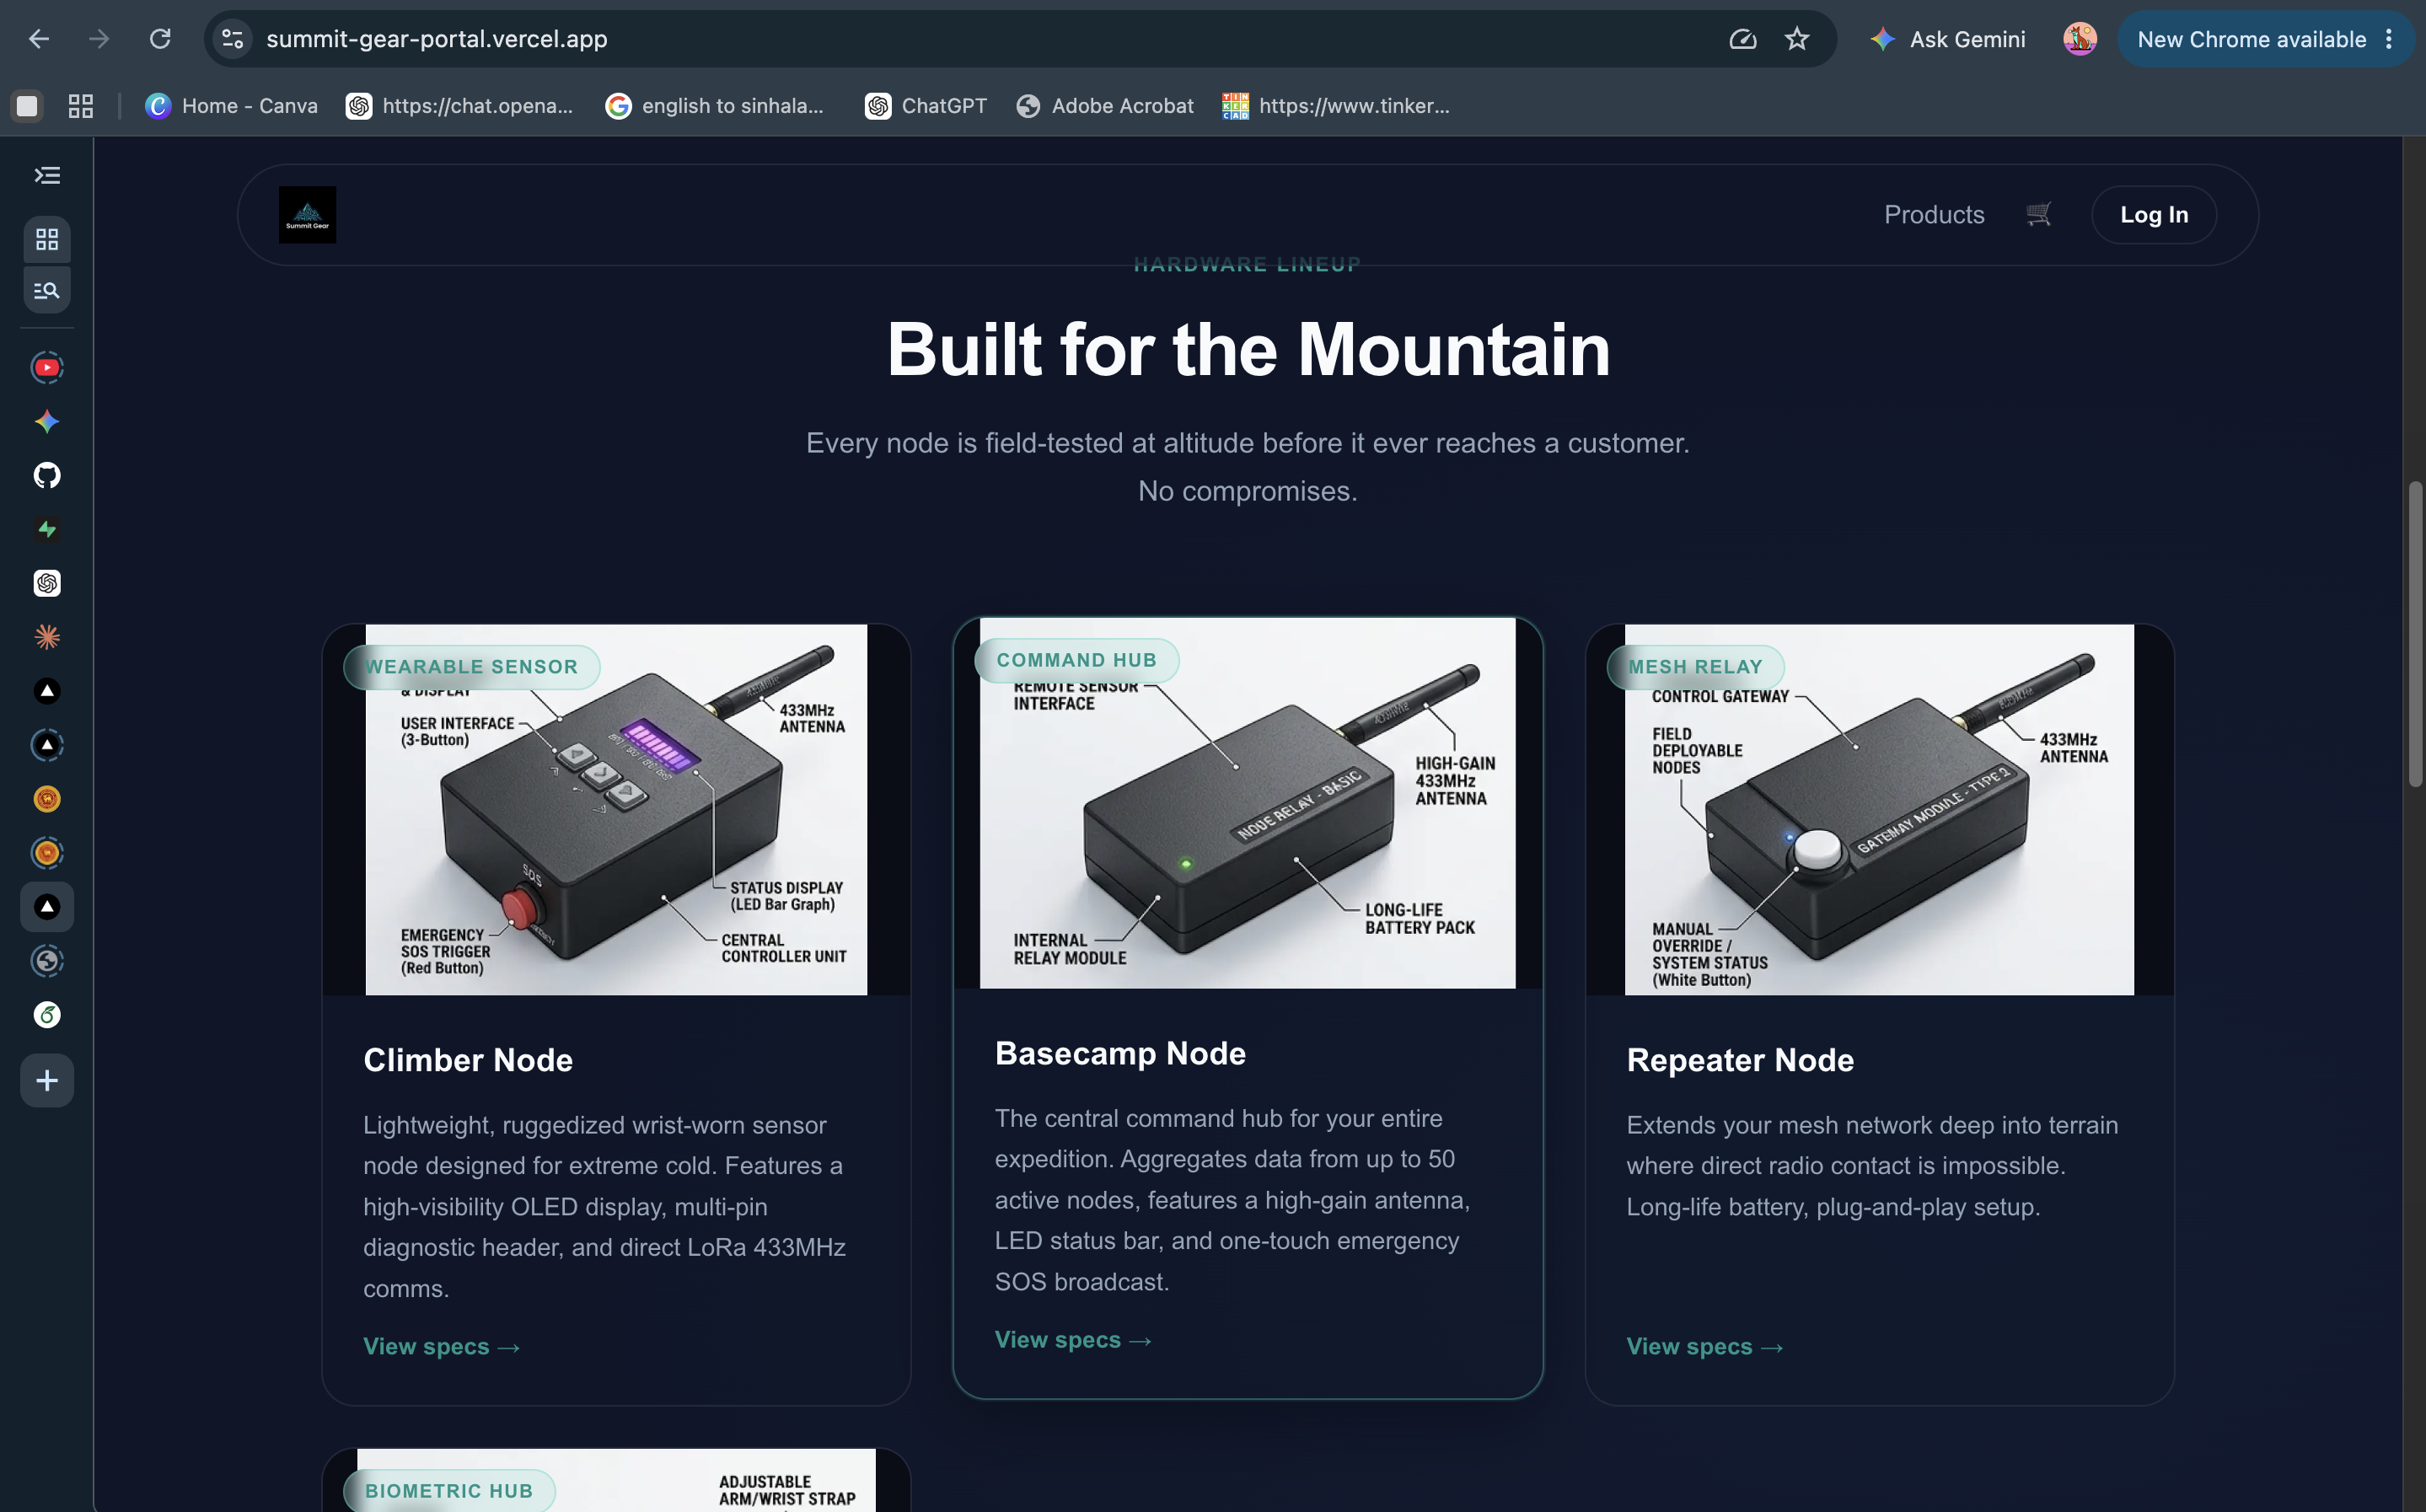
\includegraphics[width=0.8\textwidth]{figures/portal-devices.png}
    \caption{My Devices Dashboard showing registered gear}
    \label{fig:portal-devices}
\end{figure}

\subsection{Downloading Firmware and the Mobile App}
The portal provides secure access to software downloads tailored to your registered devices.

\begin{enumerate}
    \item Go to the \textbf{Downloads} section in your user dashboard.
    \item \textbf{Mobile App:} Find the links to download the latest iOS and Android versions of the Climber app.
    \item \textbf{Firmware:} Locate your registered device in the list. The portal will display the latest available firmware version (\texttt{.bin} file) for download. This file can be used for OTA updates via the mobile app or manual flashing via USB.
\end{enumerate}

\section{Administrative Operations}

\subsection{Admin Panel}
Authorized administrators can access the admin panel to manage products, orders, customers, and registered devices. It provides a comprehensive overview of system metrics and user activity.

\begin{figure}[H]
    \centering
    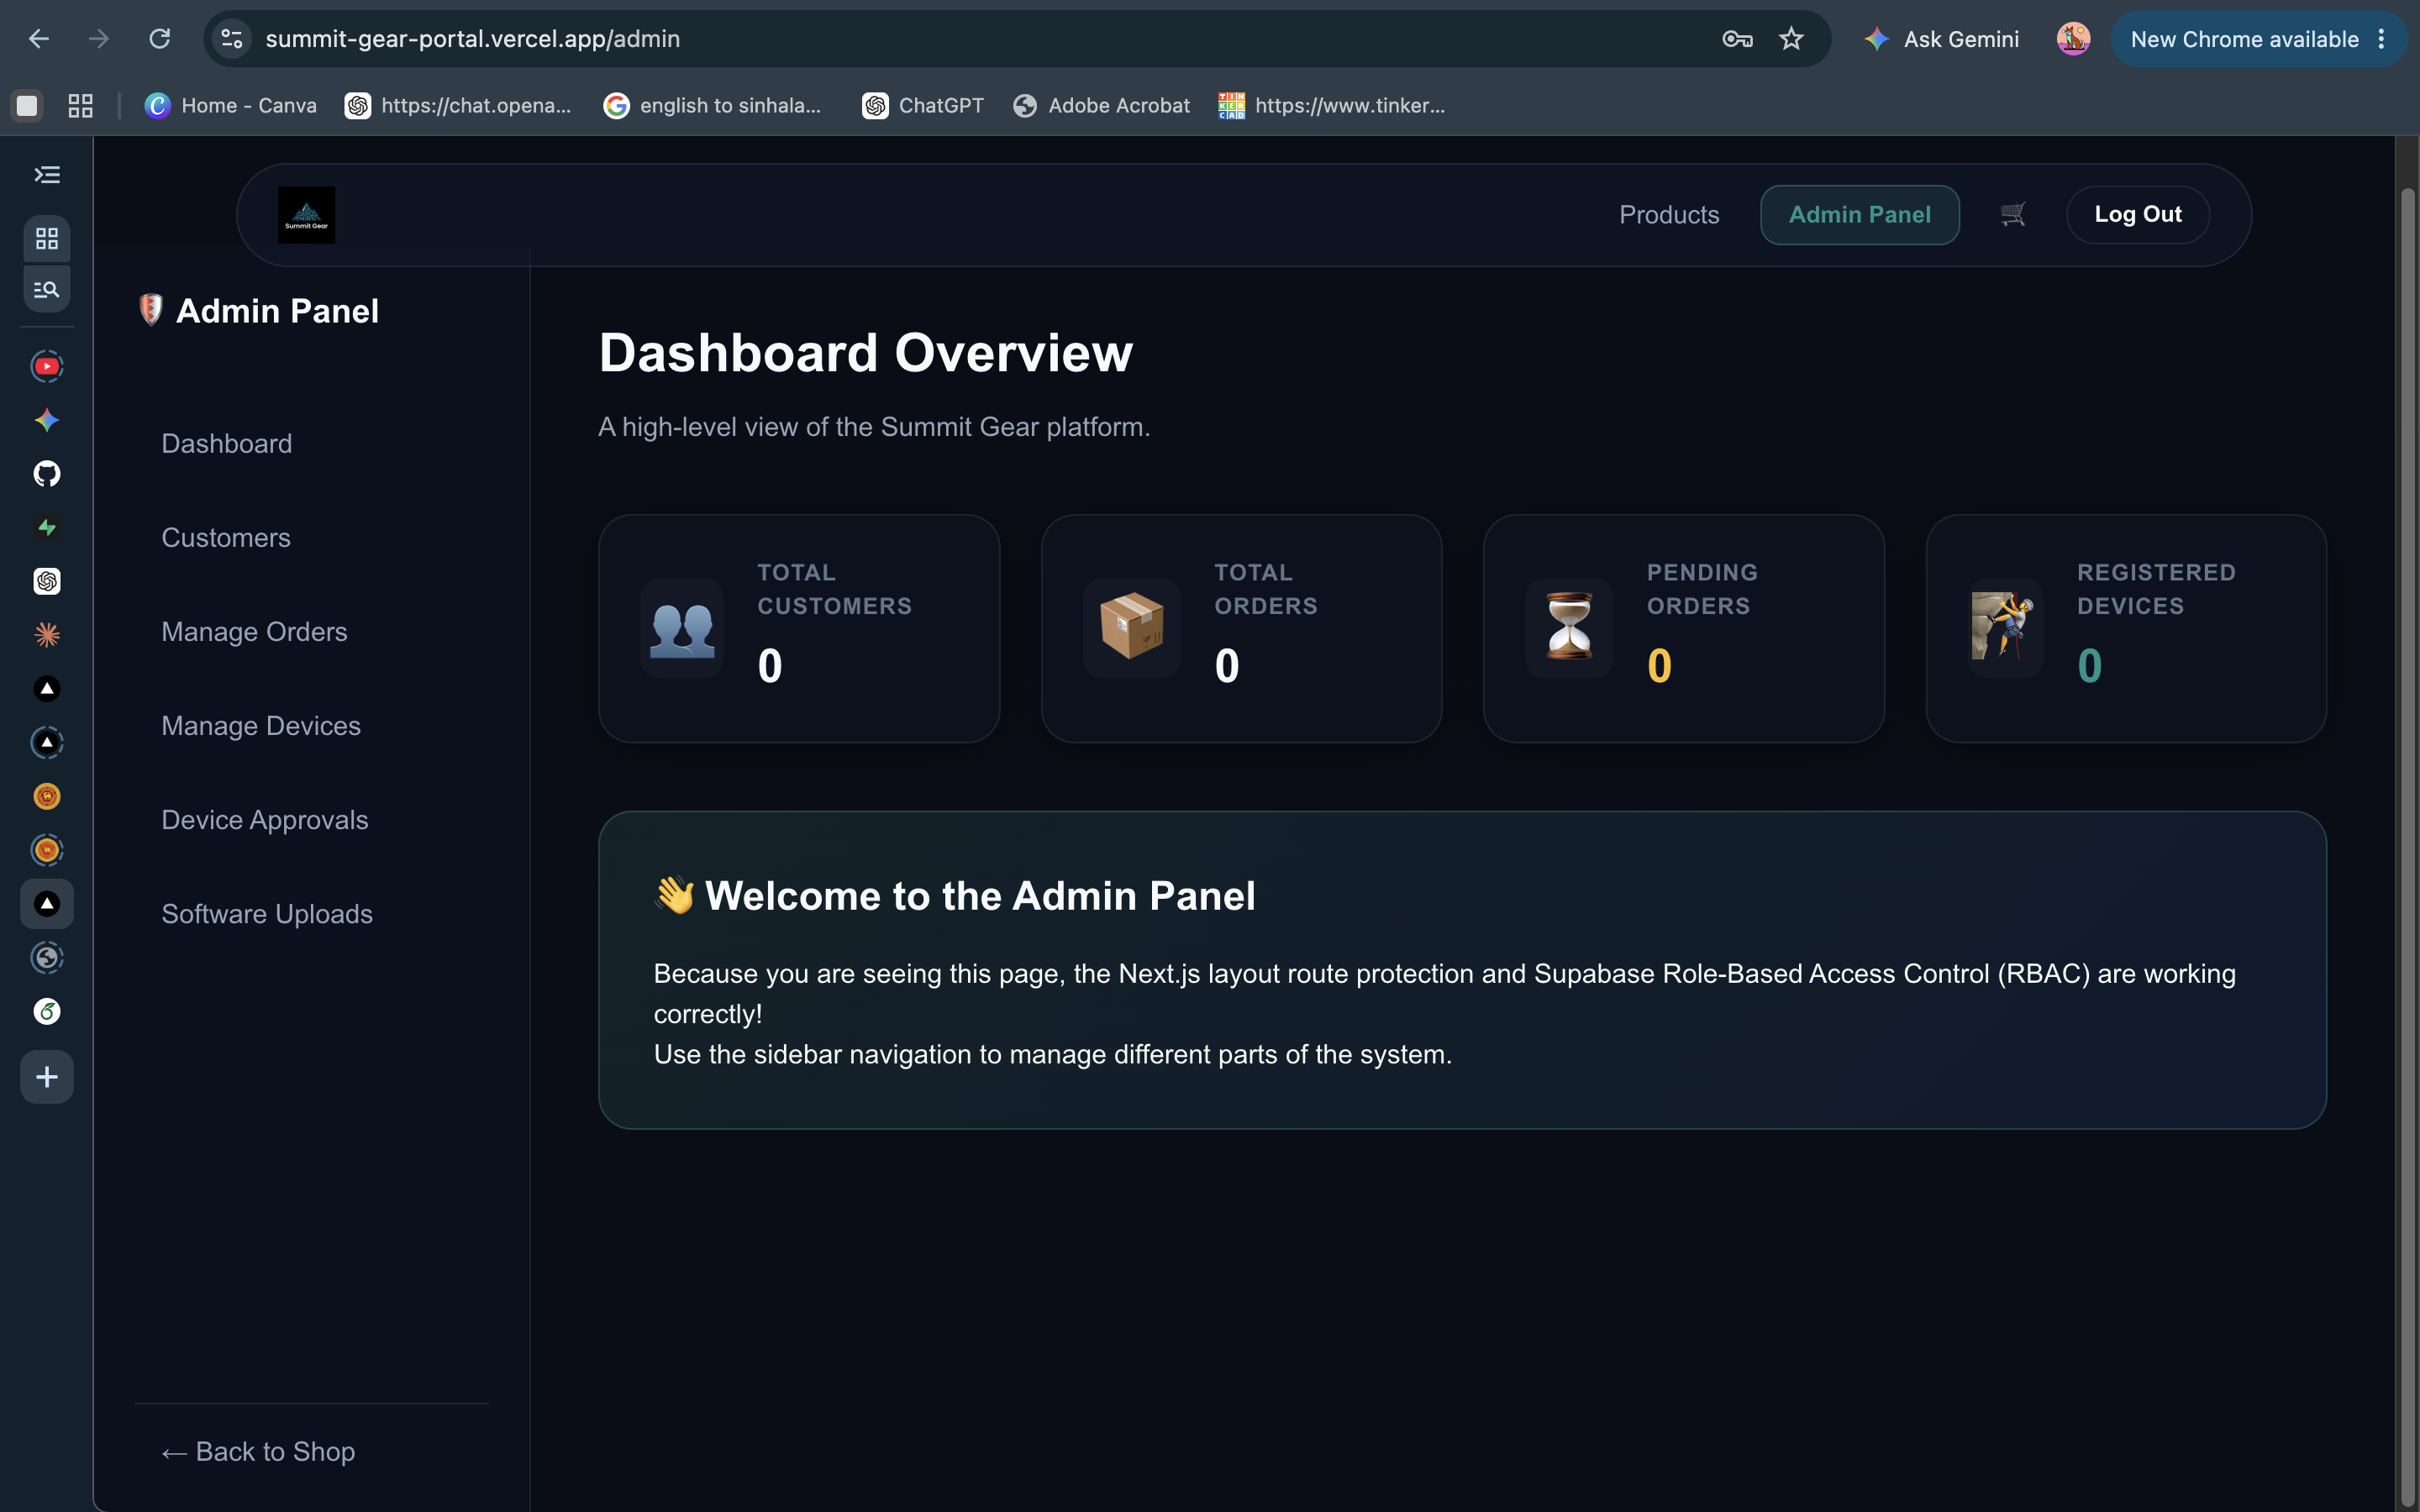
\includegraphics[width=0.9\textwidth]{figures/portal-admin-panel.png}
    \caption{Summit Gear Portal Admin Panel Interface}
    \label{fig:portal-admin-panel}
\end{figure}

\section{Account Management}

\subsection{Accessing Order History}
You can review past purchases and download invoices at any time.

\begin{enumerate}
    \item Navigate to \textbf{Account Settings > Order History}.
    \item You will see a chronological list of all your orders.
    \item Click \textbf{View Details} next to an order to see the itemized list, shipping status, and a link to download the PDF receipt.
\end{enumerate}
